\lab{Markov Chains}{Markov Chains}
\label{lab:Markov}
\objective{
A \emph{Markov chain} is a collection of states with specified probabilities for transitioning from one state to another.
They are characterized by the fact that the future behavior of the system depends only on its current state.
Markov chains have far ranging applications.
In this lab, we learn to construct, analyze, and interact with Markov chains and apply a Markov chain to natural language processing.}

\section*{State Space Models} % ===============================================

Many systems can be described by a finite number of states.
For example, a board game where players move around the board based on die rolls can be modeled by a Markov chain.
Each space represents a state, and a player is said to be in a state if their piece is currently on the corresponding space.
In this case, the probability of moving from one space to another only depends on the players current location: where the player was on a previous turn does not affect their current turn.

% A Markov chain is a collection of states, together with the probabilities of moving from one state to another.
Finite Markov chains have an associated \emph{transition matrix} that stores the information about the transitions between the states in the chain.
The $(ij)^{th}$ entry of the matrix gives the probability of moving from state $i$ to state $j$.
Thus the rows of the transition matrix must sum to 1.

\begin{info} % Row / column stochasticity
A transition matrix where the rows sum to 1 is called \emph{row stochastic} (or \emph{right stochastic}).
The columns of a \emph{column stochastic} (or \emph{left stochastic}) transition matrix each sum to 1 and the $(i,j)^{th}$ entry of the matrix gives the probability of moving from state $j$ to state $i$.
Both representations are common, but in this lab we exclusively use row stochastic transition matrices for consistency.
\end{info}

Consider a very simple weather model where the probability of being hot or cold depends on the weather of the previous day.
If the probability that tomorrow is hot given that today is hot is 0.7, and the probability that tomorrow is cold given that today is cold is 0.4, then by assigning hot to the $0^{th}$ row and column, and cold to the $1^{st}$ row and column, this Markov chain has the following transition matrix:
%
\begin{align*}
\begin{blockarray}{ccc}
& \text{\textcolor{red}{hot tomorrow}} & \text{\textcolor{blue}{cold tomorrow}} \\
\begin{block}{c(cc)}
\text{\textcolor{red}{hot today}}   & 0.7 & 0.3 \\
\text{\textcolor{blue}{cold today}} & 0.6 & 0.4 \\
\end{block}\end{blockarray}
\end{align*}

If it is hot today, we examine the $0^{th}$ row of the matrix.
There is a $70\%$ chance that tomorrow will be hot ($0^{th}$ column) and a $30\%$ chance that tomorrow will be cold ($1^{st}$ column).
Conversely, if it is cold today, there is a $60\%$ chance that tomorrow will be hot and a $40\%$ chance that tomorrow will be cold.

Markov chains can be represented by a \emph{state diagram}, a type of directed graph.
The nodes in the graph are the states, and the edges indicate the state transition probabilities.
The Markov chain described above has the following state diagram.
%
% TODO: Turn this into a tikzpicture.
\begin{figure}[H]
    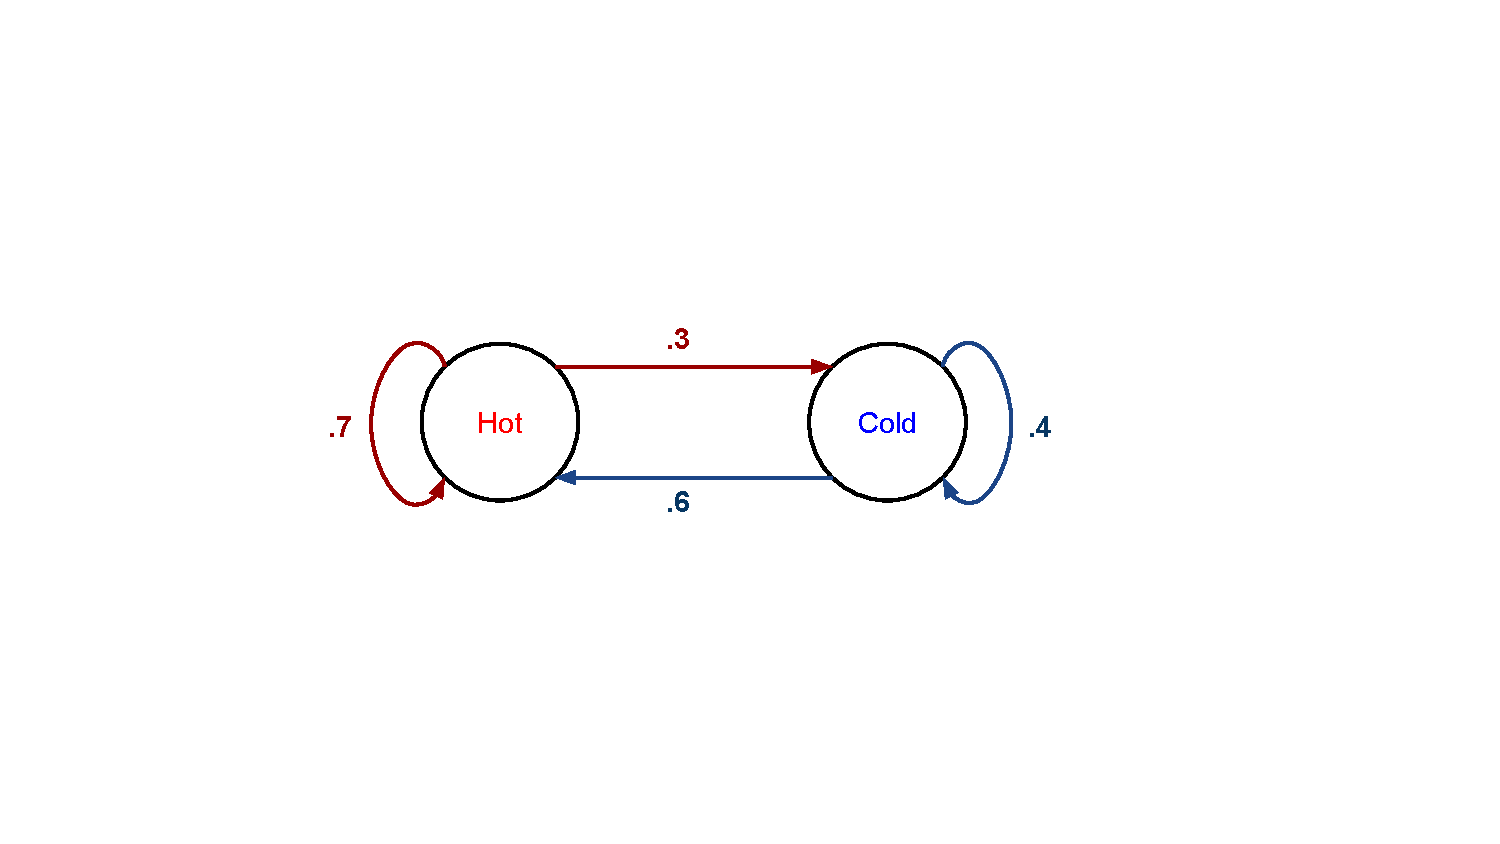
\includegraphics[width=.5\linewidth]{figures/WeatherChain.pdf}
\end{figure}
%
\begin{problem} % Problem: stochasticity.
Transition matrices for Markov chains are efficiently stored as NumPy arrays.
Write a function that accepts a dimension $n$ and returns the transition matrix for a random Markov chain with $n$ states.
\\
(Hint: use array broadcasting to avoid looping.)
\end{problem}

\subsection*{Simulating State Transitions} % ----------------------------------

% TODO: Use the binomial distribution instead of uniform. (?)
Since the rows of a transition matrix sum to $1$, the entries of each row partition the interval $[0, 1]$.
We can thus choose the next state to move to by generating a random number between $0$ and $1$.

Consider again the simple weather model and suppose that today is hot.
The row that corresponds to ``hot''in the transition matrix is $[0.7, 0.3]$.
If we generate a random number and it is smaller than $0.3$, then the simulation indicates that tomorrow will be cold.
Conversely, if the random number is between $0.3$ and $1$, then the simulation says that tomorrow will be hot.

\begin{lstlisting}
import numpy as np

def forecast():
	"""Forecast tomorrow's weather given that today is hot."""
	transition_matrix = np.array([[0.7, 0.3], [0.6, 0.4]])
	# Sample from the standard uniform distribution to choose a new state.
	if np.random.random() < transition_matrix[0, 1]:
		return 1              # Tomorrow will be cold.
	else:
		return 0              # Tomorrow will be hot.
\end{lstlisting}

\begin{problem} % Problem: Forecasting over several days.
Modify \li{forecast()} so that it accepts a parameter \li{days} and runs a simulation of the weather for the number of days given.
Return a list containing the day-by-day weather predictions (0 for hot, 1 for cold).
Assume the first day is hot, but do not include the data from the first day in the list of predictions.
The resulting list should therefore have \li{days} entries.
\end{problem}

\subsection*{Larger Chains} % -------------------------------------------------

The \li{forecast()} function makes one random draw from a \emph{uniform} distribution to simulate a state change.
Larger Markov chains require draws from a \emph{multinomial} distribution, a multivariate generalization of the binomial distribution.

A single draw from a binomial distribution with parameter $p$ indicates successes or failure of a single experiment with probability $p$ of success.
The classic example is a coin flip, where the $p$ is the probability that the coin lands heads side up.
A single draw from a multinomial distribution with parameters $\left(p_1, p_2, ..., p_n \right)$ indicates which of $n$ outcomes occurs.
In this case the classic example is a dice roll, with $6$ possible outcomes instead of the $2$ in a coin toss.

\begin{lstlisting}
# To simulate a single dice roll, store the probabilities of each outcome.
>>> die_probabilities = np.array([1./6, 1./6, 1./6, 1./6, 1./6, 1./6])

# Make a single random draw (roll the die once).
>>> np.random.multinomial(1, die_probabilities)
array([0, 0, 0, 1, 0, 0])                       # The roll resulted in a 4.
\end{lstlisting}

\begin{problem} % Problem: 4 states instead of 2. Multinomial transitioning.
Let the following be the transition chain for a Markov chain modeling weather with four states: hot, mild, cold, and freezing.

\begin{align*}
\begin{blockarray}{ccccc}
& \text{\textcolor{red}{hot}} & \text{\textcolor[rgb]{0,.6,0}{mild}} & \text{\textcolor{blue}{cold}} & \text{\textcolor{cyan}{freezing}} \\
\begin{block}{c(cccc)}
\text{\textcolor{red}{hot}}                 & 0.5 & 0.3 & 0.2 & 0 \\
\text{\textcolor[rgb]{0,.6,0}{mild}}       & 0.3 & 0.3 & 0.3 & 0.1 \\
\text{\textcolor{blue}{cold}}               & 0.1 & 0.3 & 0.4 & 0.2 \\
\text{\textcolor{cyan}{freezing}}           & 0 & 0.3 & 0.5 & 0.2 \\
\end{block}\end{blockarray}
\end{align*}

Write a new function that accepts a parameter \li{days} and runs the same kind of simulation as \li{forecast()}, but that uses this new four-state transition matrix.
This time, assume the first day is mild.
Return a list containing the day-to-day results (0 for hot, 1 for mild, 2 for cold, and 3 for freezing).
\label{prob:makov-state-transition}
\end{problem}

% TODO: instead of crappy empirical analysis, teach briefly about steady states and raising the transition matrix to a large power.

\begin{problem} % Problem: Analysis of results.
Write a function that investigates and interprets the results of the simulations in the previous two problems.
Specifically, find the average percentage of days that are hot, mild, cold, and freezing in each simulation.
Does changing the starting day alter the results?
Print a report of your findings.
\end{problem}

\section*{Using Markov Chains to Simulate English} % ==========================
% TODO: is it okay to make this reference?
One of the original applications of Markov chains was to study natural languages.\footnote{In computer science, a \emph{natural language} is a spoken language, like English or Russian. See \url{http://langvillea.people.cofc.edu/MCapps7.pdf} for some details on the early applications of Markov chains, including the study of natural languages.}
In the early $20^{th}$ century, Markov used his chains to model how Russian switched from vowels to consonants.
By mid-century, they had been used as an attempt to model English.
It turns out that Markov chains are, by themselves, insufficient to model very good English.
However, they can approach a fairly good model of bad English, with sometimes amusing results.

By nature, a Markov chain is only concerned with its current state.
Thus a Markov chain simulating transitions between English words is completely unaware of context or even of previous words in a sentence.
For example, a Markov chain's current state may be the word ``continuous.''
Then the chain would say that the next word in the sentence is more likely to be ``function'' rather than ``raccoon.''
However, without the context of the rest of the sentence, even two likely words stringed together may result in gibberish.

We restrict ourselves to a subproblem of modeling the English of a specific file.
The transition probabilities of the resulting Markov chain will reflect the sort of English that the source authors speak.
Thus the Markov chain built from \emph{The Complete Works of William Shakespeare} will differ greatly from, say, the Markov chain built from a collection of academic journals.
We will call the source collection of works in the next problems the \emph{training set}.

\subsection*{Making the Chain} % ----------------------------------------------

With the weather models of the previous sections, we chose a fixed number of days to simulate.
However, English sentences are of varying length, so we do not know beforehand how many words to choose (how many state transitions to make) before ending the sentence.
To capture this feature, we include two extra states in our Markov model: a \emph{start state} (\textcolor[rgb]{0,.6,0}{\$tart}) marking the beginning of a sentence, and a \emph{stop state} (\textcolor{red}{\$top}) marking the end.
Thus if a training set has $N$ unique words, the transition matrix will be $(N+2) \times (N+2)$.

The start state should only transition to words that appear at the beginning of a sentence in the training set, and only words that appear at the end a sentence in the training set should transition to the stop state.
The stop state is called an \emph{absorbing state} because once we reach it, we cannot transition back to another state.
% Because every state has a possible path to the stop state, this model is called an \emph{absorbing Markov chain}.

After determining the states in the Markov chain, we need to determine the transition probabilities between the states and build the corresponding transition matrix.
Consider the following small training set as an example.

\begin{lstlisting}
<<I am Sam Sam I am.
Do you like green eggs and ham?
I do not like them, Sam I am.
I do not like green eggs and ham.>>
\end{lstlisting}

If we include punctuation (so ``ham?'' and ``ham.'' are counted as distinct words) and do not alter the capitalization (so ``Do'' and ``do'' are also different), there are 15 unique words in this training set:
%
\begin{align*}
\text{I\quad am\quad Sam\quad am.\quad Do\quad you\quad like\quad green}
\\
\text{eggs\quad and\quad ham?\quad do\quad not\quad them,\quad ham.}
\end{align*}

With start and stop states, the transition matrix should be $17 \times 17$.
Each state must be assigned a row and column index in the transition matrix.
As easy way to do this is to assign the states an index based on the order that they appear in the training set.
Thus our states and the corresponding indices will be as follows:
%
\begin{align*}
\begin{array}{ccccccc}
\text{\textcolor[rgb]{0,.6,0}{\$tart}} & \text{I} & \text{am} & \text{Sam} & \ldots & \text{ham.} & \text{\textcolor{red}{\$top}}
\\
0 & 1 & 2 & 3 & \ldots & 15 & 16
\end{array}
\end{align*}

The start state should transition to the words ``I'' and ``Do'', and the words ``am.'', ``ham?'', and ``ham.'' should each transition to the stop state.
We first count the number of times that each state transitions to another state:

\begin{align*}
\begin{blockarray}{cccccccc}
& \text{\textcolor[rgb]{0,.6,0}{\$tart}} & \text{I} & \text{am} & \text{Sam} & & \text{ham.} & \text{\textcolor{red}{\$top}} \\
\begin{block}{c(ccccccc)}
\text{\textcolor[rgb]{0,.6,0}{\$tart}} 	& 0 & 3 & 0 & 0 & \ldots & 0 & 0\\
\text{I} 		& 0 & 0 & 1 & 0 & \ldots & 0 & 0\\
\text{am} 		& 0 & 0 & 0 & 1 & \ldots & 0 & 0\\
\text{Sam} 		& 0 & 2 & 0 & 1 & \ldots & 0 & 0\\
& \vdots & \vdots & \vdots & \vdots & \ddots & \vdots & \vdots\\
\text{ham.} 	& 0 & 0 & 0 & 0 & \ldots & 0 & 1\\
\text{\textcolor{red}{\$top}} 		& 0 & 0 & 0 & 0 & \ldots & 0 & 1\\
\end{block}\end{blockarray}
\end{align*}

Now we divide each row by its sum so that each row sums to 1.

\begin{align*}
\begin{blockarray}{cccccccc}
& \text{\textcolor[rgb]{0,.6,0}{\$tart}} & \text{I} & \text{am} & \text{Sam} & & \text{ham.} & \text{\textcolor{red}{\$top}} \\
\begin{block}{c(ccccccc)}
\text{\textcolor[rgb]{0,.6,0}{\$tart}} & 0 & 3/4 & 0 & 0 & \ldots & 0 & 0\\
\text{I}        & 0 & 0 & 1/5 & 0 & \ldots & 0 & 0\\
\text{am}       & 0 & 0 & 0 & 1 & \ldots & 0 & 0\\
\text{Sam}      & 0 & 2/3 & 0 & 1/3 & \ldots & 0 & 0\\
& \vdots & \vdots & \vdots & \vdots & \ddots & \vdots & \vdots\\
\text{ham.}     & 0 & 0 & 0 & 0 & \ldots & 0 & 1\\
\text{\textcolor{red}{\$top}}        & 0 & 0 & 0 & 0 & \ldots & 0 & 1\\
\end{block}\end{blockarray}
\end{align*}

The $3/4$ indicates that 3 out of 4 times, the sentences in the training set start with the word ``I''.
Similarly, the $2/3$ and $1/3$ tell us that ``Sam'' is followed by ``I'' twice and by ``Sam'' once in the training set.
Note that ``am'' (without a period) always transitions to ``Sam'' and that ``ham.'' (with a period) always transitions the stop state.
Finally, to avoid a row of zeros, we place a 1 in the bottom right hand corner of the matrix (so the stop state always transitions to itself).

The entire procedure of creating the transition matrix for the Markov chain with words from a file as states is summarized below in Algorithm \ref{alg:MarkovSentencesTransitionMatrix}.

\begin{algorithm} % Read a file and convert it into a Markov chain.
\begin{algorithmic}[1]
\Procedure{MakeTransitionMatrix}{}
\State Count the number of unique words in the training set.
\State Initialize a square array of zeros of the appropriate size to be the transition \par\quad matrix (remember to account for the start and stop states).
\State Initialize a list of states, beginning with \li{"\$tart"}.
\For {each sentence in the training set}
    \State Split the sentence into a list of words.
    \State Add each \emph{new} word in the sentence to the list of states.
    \State Convert the list of words into a list of indices indicating which row and \par\qquad\enspace column of the transition matrix each word corresponds to.
    \State Add 1 to the entry of the transition matrix corresponding to
    \par\qquad\enspace transitioning from the start state to the first word of the sentence.
    \For {each consecutive pair $(i, j)$ of words in the list of words}
        \State Add 1 to the entry of the transition matrix corresponding to \par\qquad\qquad transitioning from state $i$ to state $j$.
    \EndFor
    \State Add 1 to the entry of the transition matrix corresponding to
    \par\qquad\enspace transitioning from the last word of the sentence to the stop state.
\EndFor
\State Make sure the stop state transitions to itself.
\State Normalize each row by dividing by the row sums (Hint: array broadcasting).
\EndProcedure
\end{algorithmic}
\caption{Convert a training set of sentences into a Markov chain.}
\label{alg:MarkovSentencesTransitionMatrix}
\end{algorithm}

\begin{problem} % Problem: Class that makes a Markov chain from a file.
Write a class called \li{SentenceGenerator}.
The constructor should accept a filename (the training set).
Read the file and build a transition matrix from its contents.
You may assume that the file has one complete sentence written on each line.
\label{problem:markov-random-sentences-init}
\end{problem}

\begin{problem} % Problem: Create random sentences
Add a method to the \li{SentenceGenerator} class called \li{babble()}.
Begin at the start state and use the strategy from Problem \ref{prob:makov-state-transition} to repeatedly transition through the object's Markov chain.
Keep track of the path through the chain and the corresponding sequence of words.
When the stop state is reached, stop transitioning to terminate the simulation.
Return the resulting sentence as a single string.
\newpage
For example, your \li{SentenceGenerator} class should be able to create random sentences that sound somewhat like Yoda speaking.

\begin{lstlisting}
>>> yoda = SentenceGenerator("Yoda.txt")
>>> for i in xrange(5):
... 	print(yoda.babble())
...
<<
Impossible to my size, do not!
For eight hundred years old to enter the dark side of Congress there is.
But beware of the Wookiees, I have.
Fear leads to eat as well.
But agree on this, we must, and find your weapon!>>
\end{lstlisting}

\label{prob:markov-random-sentences-babble}
\end{problem}

\newpage

\section*{Additional Material} % ==============================================

\subsection*{Large Training Sets} % -------------------------------------------

The approach in Problems \ref{problem:markov-random-sentences-init} and \ref{prob:markov-random-sentences-babble} begins to fail as the training set grows larger.
For example, a single Shakespearean play may not be large enough to cause memory problems, but \emph{The Complete Works of William Shakespeare} certainly will.

To accommodate larger data sets, consider use a sparse matrix for the transition matrix in instead of a regular NumPy array. %(use the \li{lil_matrix} from the \li{scipy.sparse} library). % Why lil_matrix?
Ensure that the process still works on small training sets, then proceed to larger training sets.
How are the resulting sentences different if a very large training set is used instead of a small training set?

\subsection*{Variations on the English Model} % -------------------------------

Choosing a different state space for the English Markov model produces different results.
Consider modifying your \li{SentenceGenerator} class so that it can determine the state space in a few different ways.
The following ideas are just a few possibilities.

\begin{itemize}
\item Let each punctuation mark have its own state.
In the example training set, instead of having two states for the words ``ham?'' and ``ham.'', there would be three states: ``ham'', ``?'', and ``.'', with ``ham'' transitioning to both punctuation states.
\item Model paragraphs instead of sentences.
Add a \textcolor[rgb]{0,.6,0}{\$tartParagraph} state that always transitions to \textcolor[rgb]{0,.6,0}{\$tartSentence} and a \textcolor{red}{\$topParagraph} state that is sometimes transitioned to from \textcolor{red}{\$topSentence}.
\item Let the states be individual letters instead of individual words.
Be sure to include a state for the spaces between words.
We will explore this particular state space choice more in Volume III.
\end{itemize}

\subsection*{Natural Language Processing Tools} % -----------------------------

The Markov model of Problems \ref{problem:markov-random-sentences-init} and \ref{prob:markov-random-sentences-babble} is an example of \emph{natural language processing}.
The \li{nltk} module (natural language toolkit) has many tools for parsing and analyzing text.
For example, \li{nltk.sent_tokenize()} reads a single string and splits it up by sentence.

\begin{lstlisting}
>>> from nltk import sent_tokenize
>>> with open("Yoda.txt", 'r') as yoda:
...     sentences = sent_tokenize(yoda.read())
...
>>> print(sentences)
<<['Away with your weapon!',
 'I mean you no harm.',
 'I am wondering - why are you here?',
 ...>>
\end{lstlisting}

The \li{nltk} module is \textbf{not} part of the Python standard library.
For instructions on downloading, installing, and using \li{nltk}, visit \url{http://www.nltk.org/}.
